\documentclass[border=15pt]{standalone}
\usepackage{amsmath, amssymb}
\usepackage{tikz}
\usetikzlibrary{arrows.meta}

\definecolor{block0}{HTML}{E53935}
\definecolor{block1}{HTML}{1E88E5}

\begin{document}
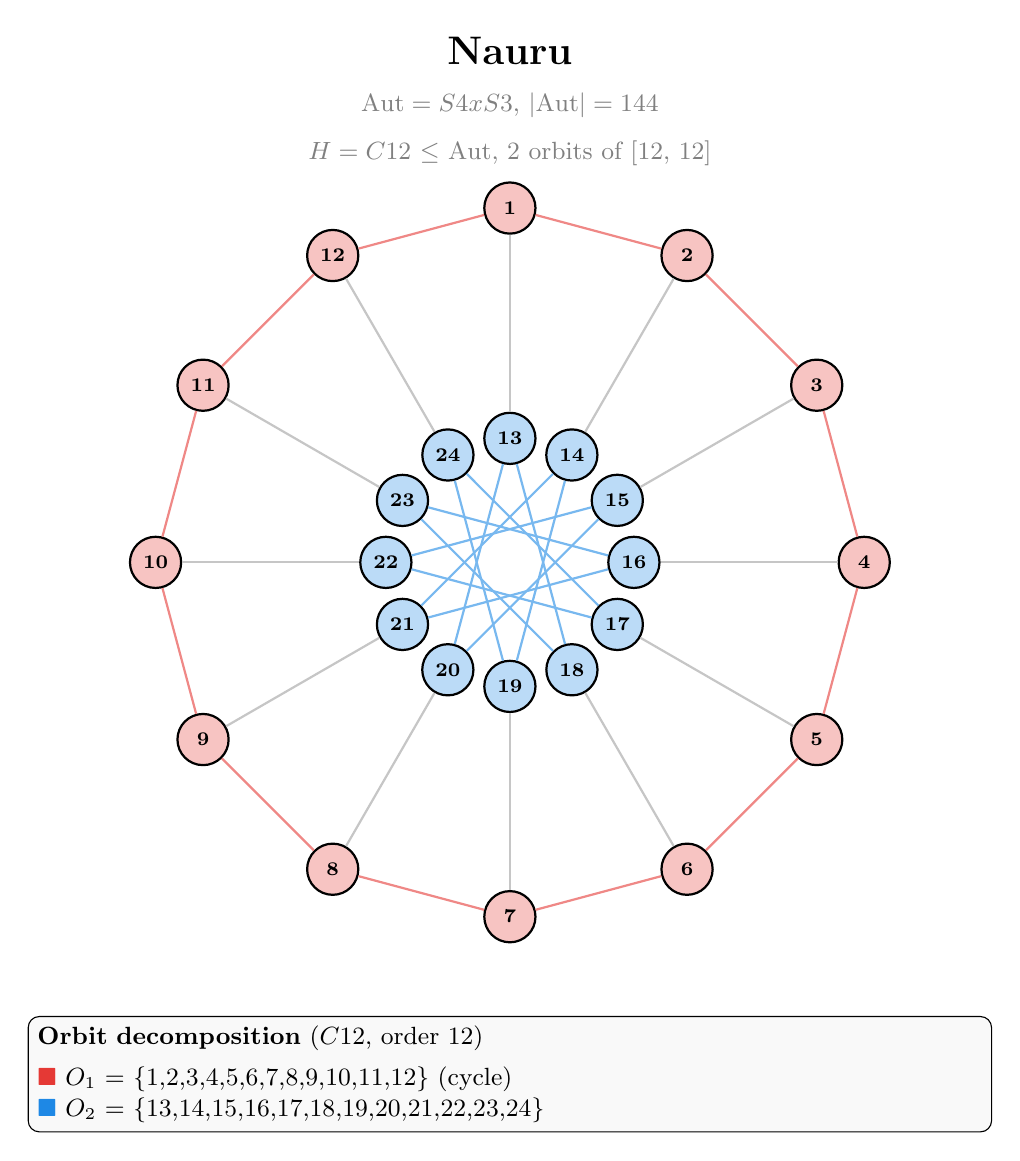
\begin{tikzpicture}[
  vertex/.style={circle, draw, thick, minimum size=6.5mm, inner sep=0pt,
                 font=\scriptsize\bfseries},
  edge/.style={thick, gray!45},
  title/.style={font=\Large\bfseries},
  subtitle/.style={font=\small, text=gray},
]

\node[title] at (0, 6.5) {Nauru};
\node[subtitle] at (0, 5.8) {$\mathrm{Aut} = S4 x S3$, $|\mathrm{Aut}| = 144$};
\node[subtitle] at (0, 5.2) {$H = C12$ $\leq$ $\mathrm{Aut}$, 2 orbits of [12, 12]};

\node[vertex, fill=block0!30] (v1) at (0.000, 4.500) {1};
\node[vertex, fill=block0!30] (v2) at (2.250, 3.897) {2};
\node[vertex, fill=block0!30] (v3) at (3.897, 2.250) {3};
\node[vertex, fill=block0!30] (v4) at (4.500, -0.000) {4};
\node[vertex, fill=block0!30] (v5) at (3.897, -2.250) {5};
\node[vertex, fill=block0!30] (v6) at (2.250, -3.897) {6};
\node[vertex, fill=block0!30] (v7) at (-0.000, -4.500) {7};
\node[vertex, fill=block0!30] (v8) at (-2.250, -3.897) {8};
\node[vertex, fill=block0!30] (v9) at (-3.897, -2.250) {9};
\node[vertex, fill=block0!30] (v10) at (-4.500, 0.000) {10};
\node[vertex, fill=block0!30] (v11) at (-3.897, 2.250) {11};
\node[vertex, fill=block0!30] (v12) at (-2.250, 3.897) {12};
\node[vertex, fill=block1!30] (v13) at (0.000, 1.575) {13};
\node[vertex, fill=block1!30] (v14) at (0.787, 1.364) {14};
\node[vertex, fill=block1!30] (v15) at (1.364, 0.788) {15};
\node[vertex, fill=block1!30] (v16) at (1.575, -0.000) {16};
\node[vertex, fill=block1!30] (v17) at (1.364, -0.788) {17};
\node[vertex, fill=block1!30] (v18) at (0.788, -1.364) {18};
\node[vertex, fill=block1!30] (v19) at (-0.000, -1.575) {19};
\node[vertex, fill=block1!30] (v20) at (-0.788, -1.364) {20};
\node[vertex, fill=block1!30] (v21) at (-1.364, -0.788) {21};
\node[vertex, fill=block1!30] (v22) at (-1.575, 0.000) {22};
\node[vertex, fill=block1!30] (v23) at (-1.364, 0.787) {23};
\node[vertex, fill=block1!30] (v24) at (-0.787, 1.364) {24};

\draw[thick, block0!60] (v1) -- (v2);
\draw[thick, block0!60] (v1) -- (v12);
\draw[edge] (v1) -- (v13);
\draw[thick, block0!60] (v2) -- (v3);
\draw[edge] (v2) -- (v14);
\draw[thick, block0!60] (v3) -- (v4);
\draw[edge] (v3) -- (v15);
\draw[thick, block0!60] (v4) -- (v5);
\draw[edge] (v4) -- (v16);
\draw[thick, block0!60] (v5) -- (v6);
\draw[edge] (v5) -- (v17);
\draw[thick, block0!60] (v6) -- (v7);
\draw[edge] (v6) -- (v18);
\draw[thick, block0!60] (v7) -- (v8);
\draw[edge] (v7) -- (v19);
\draw[thick, block0!60] (v8) -- (v9);
\draw[edge] (v8) -- (v20);
\draw[thick, block0!60] (v9) -- (v10);
\draw[edge] (v9) -- (v21);
\draw[thick, block0!60] (v10) -- (v11);
\draw[edge] (v10) -- (v22);
\draw[thick, block0!60] (v11) -- (v12);
\draw[edge] (v11) -- (v23);
\draw[edge] (v12) -- (v24);
\draw[thick, block1!60] (v13) -- (v18);
\draw[thick, block1!60] (v13) -- (v20);
\draw[thick, block1!60] (v14) -- (v19);
\draw[thick, block1!60] (v14) -- (v21);
\draw[thick, block1!60] (v15) -- (v20);
\draw[thick, block1!60] (v15) -- (v22);
\draw[thick, block1!60] (v16) -- (v21);
\draw[thick, block1!60] (v16) -- (v23);
\draw[thick, block1!60] (v17) -- (v22);
\draw[thick, block1!60] (v17) -- (v24);
\draw[thick, block1!60] (v18) -- (v23);
\draw[thick, block1!60] (v19) -- (v24);

\node[draw, rounded corners, fill=gray!5, text width=12cm, align=left, font=\small]
  at (0, -6.5) {
  \textbf{Orbit decomposition} ($C12$, order 12) \\[4pt]
  \textcolor{block0}{$\blacksquare$} $O_{1}$ = \{1,2,3,4,5,6,7,8,9,10,11,12\} (cycle) \\
  \textcolor{block1}{$\blacksquare$} $O_{2}$ = \{13,14,15,16,17,18,19,20,21,22,23,24\}
};

\end{tikzpicture}
\end{document}